\documentclass{tufte-handout}

\title{Utility Theory and the Representation of Preference}

\author[Nathaniel Forde]{Nathaniel Forde}

%\date{28 March 2010} % without \date command, current date is supplied

%\geometry{showframe} % display margins for debugging page layout

\usepackage{graphicx} % allow embedded images
  \setkeys{Gin}{width=\linewidth,totalheight=\textheight,keepaspectratio}
  \graphicspath{{graphics/}} % set of paths to search for images
\usepackage{amsmath}  % extended mathematics
\usepackage{booktabs} % book-quality tables
\usepackage{units}    % non-stacked fractions and better unit spacing
\usepackage{multicol} % multiple column layout facilities
\usepackage{lipsum}   % filler text
\usepackage{fancyvrb} % extended verbatim environments
  \fvset{fontsize=\normalsize}% default font size for fancy-verbatim environments
\usepackage{minted}
\usepackage{mathtools}
\usepackage[math]{cellspace}
\usepackage[most]{tcolorbox}
\usepackage{tikz}
\usepackage{mdframed}
\newtheorem{theo}[section]{Theorem}

\newenvironment{ftheo}[1]
  {\begin{mdframed}
  \sloppy
  \begin{theo}[#1]
  }
  {\end{theo}
\end{mdframed}}

% Standardize command font styles and environments
\newcommand{\doccmd}[1]{\texttt{\textbackslash#1}}% command name -- adds backslash automatically
\newcommand{\docopt}[1]{\ensuremath{\langle}\textrm{\textit{#1}}\ensuremath{\rangle}}% optional command argument
\newcommand{\docarg}[1]{\textrm{\textit{#1}}}% (required) command argument
\newcommand{\docenv}[1]{\textsf{#1}}% environment name
\newcommand{\docpkg}[1]{\texttt{#1}}% package name
\newcommand{\doccls}[1]{\texttt{#1}}% document class name
\newcommand{\docclsopt}[1]{\texttt{#1}}% document class option name
\newenvironment{docspec}{\begin{quote}\noindent}{\end{quote}}% command specification environment
\definecolor{myblue}{RGB}{3,81,138}
\definecolor{mygray}{RGB}{236, 236, 236}

\tcbset{mystyle/.style={
  breakable,
  enhanced,
  outer arc=0pt,
  arc=0pt,
  colframe=myblue,
  colback=mygray,
  attach boxed title to top left,
  boxed title style={
    colback=myblue,
    outer arc=0pt,
    arc=0pt,
    },
  fonttitle=\sffamily
  }
}

\newtcolorbox[auto counter,number within=chapter]{example}[1][]{
  mystyle,
  title= Box~\thetcbcounter:#1
}



\begin{document}

\maketitle% this prints the handout title, author, and date

\begin{abstract}
\noindent
This article continues the investigation of the expected utility model of rational choice. We begin by examining the useful properties of utility functions, before continuing to the representation theorems which formalise the connection. Will we see that the nature of these theorems, coupled with the indeterminacy of statistical inference is a brittle foundation for predictive economic models of consumer choice.
\end{abstract}


\section{From Utility to Indifference}
Too much of a good thing often tends to the bad. So we dabble, sample and share. In pursuit of variety we swap our goods, shunning stale options in favour of the novel exchange.  For a given good we can differ in our appetites but it's relatively straightforward to find the point where one more donut is one too many. While it can be a bit unclear how we should measure utility, once we've decided on a metric the mathematical characteristics are meaningful. We can infer aspects of your attitudes towards acquisition and enthusiasm for donuts. In most cases we're interested not just in your pursuit of pastries, but how you'd be willing to trade for those pastries. 

\begin{marginfigure}
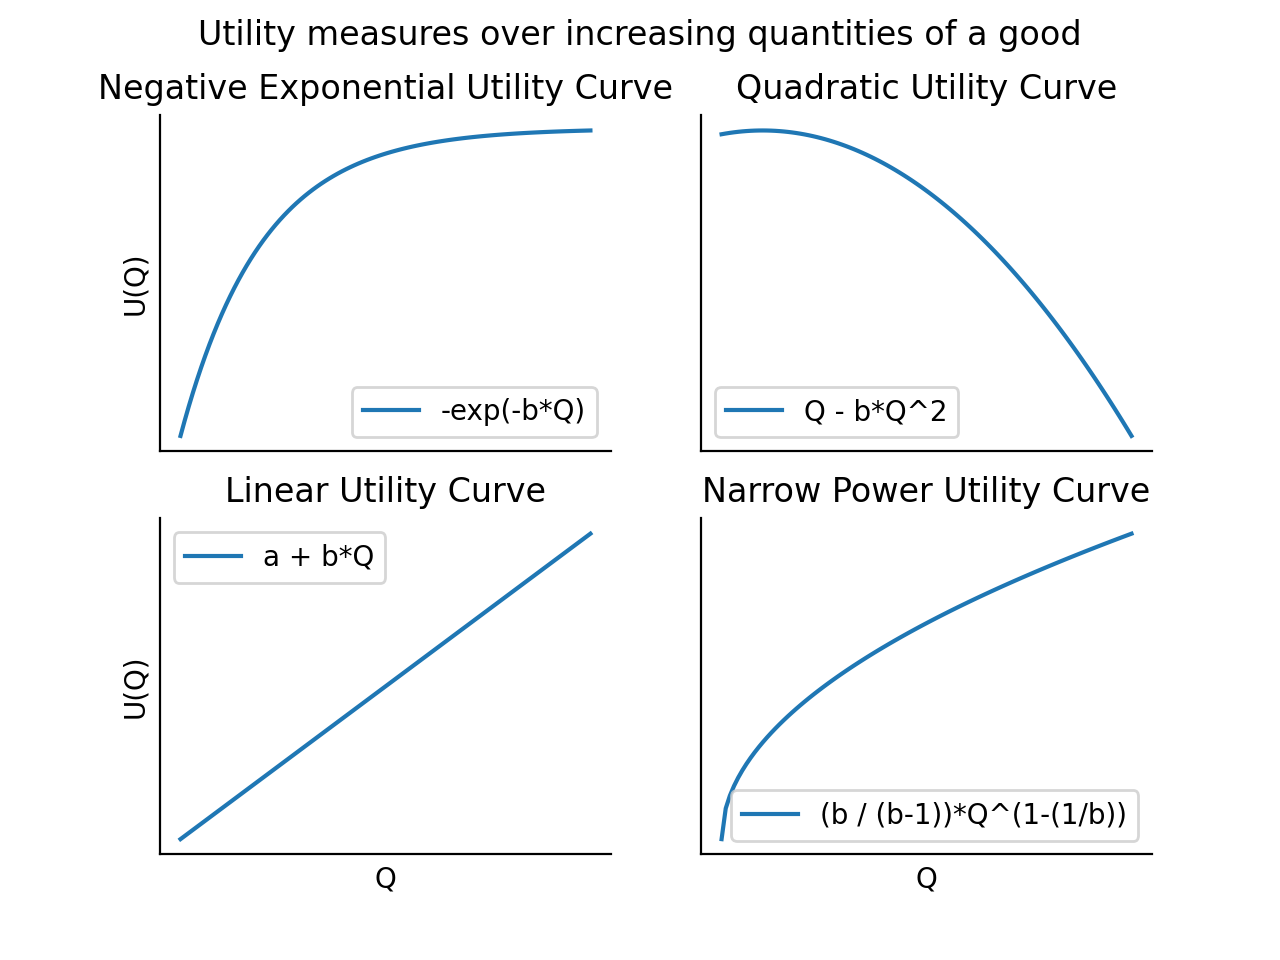
\includegraphics[width=3in]{Plots/utility_in_1_dimension.png}
\caption{Consumer attitudes with differently satisfied appetites for a good}
\includegraphics[width=3in]{Plots/derivatives_of_utility.png}
\caption{The Rates of Change of personal Utility}
\end{marginfigure} 

The possibility of coordinated compromise lies at the core of maximising subjective utility. We seek competitive advantage for our own produce to balance the cost owed to the skills of others. At the limit some trades do not admit any mixture of goods. Not all babies can be cut in half. On the other side of the spectrum, there are some things for which we'd give everything. In most cases though a consumer will try to optimise their bundle of goods over an entire marketplace, preserving enough on one key good; money, to remain liquid. 

$$ u(\mathbf{g}) = f(g_{0}, g_{1} ... g_{n}) $$

There are number of ways we can specify a utility function, but a typical example is the Cobb-Douglas function. 

$$ u(\mathbf{g}) = g_{0}^{\alpha_{0}}g_{1}^{\alpha_{1}} ... g_{n}^{\alpha_{n}}$$

\begin{marginfigure}
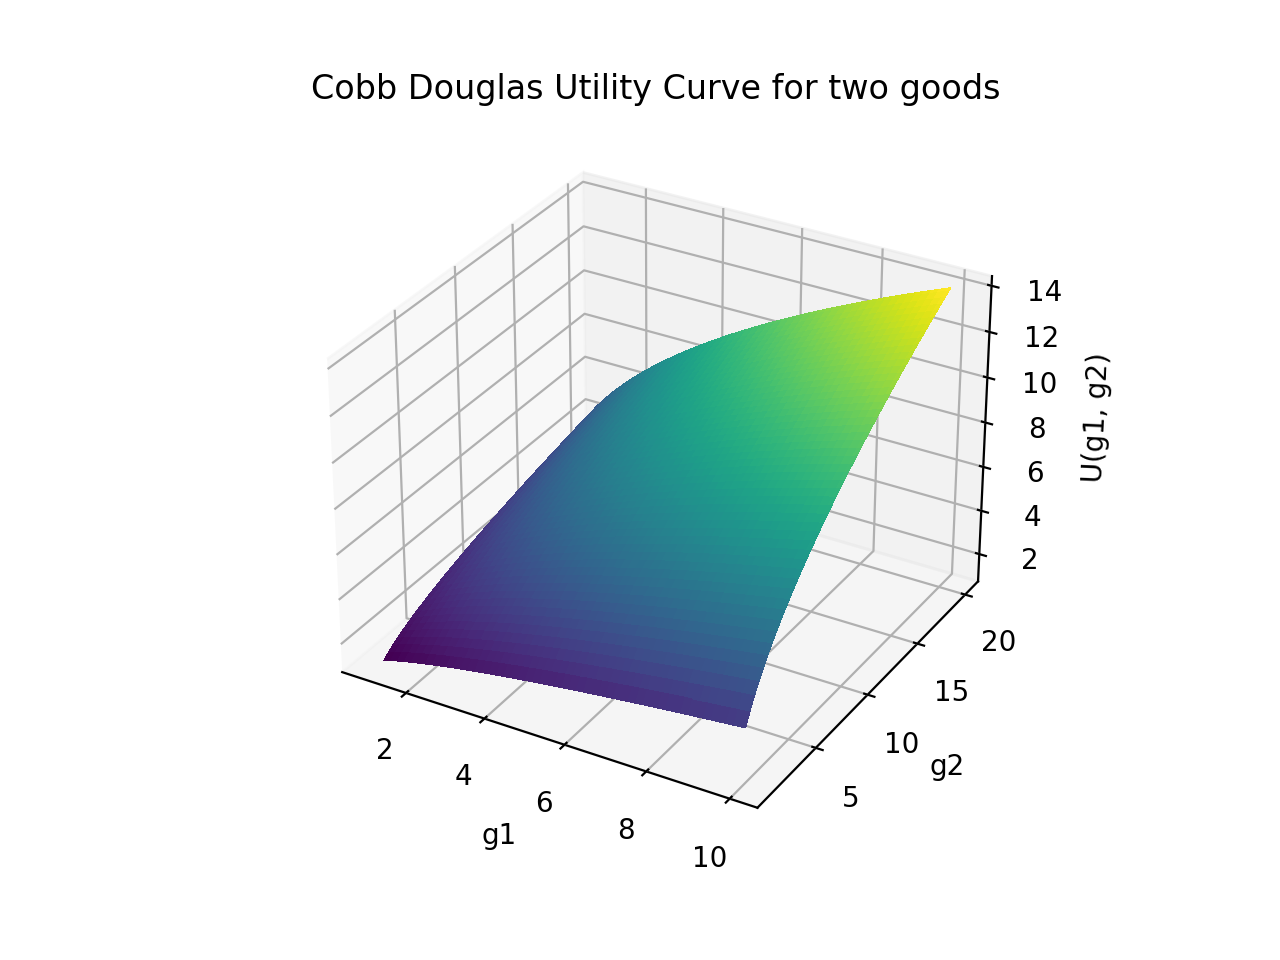
\includegraphics[width=3.2in, height=5.in]{Plots/cobb_douglas_utility.png}
\caption{A consumers utility curve for combinations of two goods}
\end{marginfigure} 

Then taking the case of two goods $g1, g2$ we can in this particular case determine an indifference curve where you would be willing to exchange quantities of $g1$ for an agreeable amount of $g2$. The task it to express the value of a given good as priced in terms of the other goods. Set 
$$u(\mathbf{g}) = \lambda =  g_{1}^{\frac{1}{2}}g_{2}^{\frac{1}{2}} = (g_{1}g_{2})^{\frac{1}{2}}  = \sqrt{g_{1}g_{2}}$$
$$ \Rightarrow \lambda^{2} = g_{1}g_{2} \Rightarrow \frac{\lambda^{2}}{g_{2}} = g_{1}$$

Using this formula we can express how the quantities of fair exchange vary based on a fixed utility value. This is not to say that these curves represent an actual or objective fair price, just that when measured in terms of utility these are mappings of quantities of good we would be happy to exchange. Your view of a fair price is encoded in your utility theory. It's at this point when utility theory can be said to verge on empirical science.If we can model your preferences as a utility function characteristic of some general attitude toward acquisition, we might also hope to able to predict future trades.  
\begin{marginfigure}
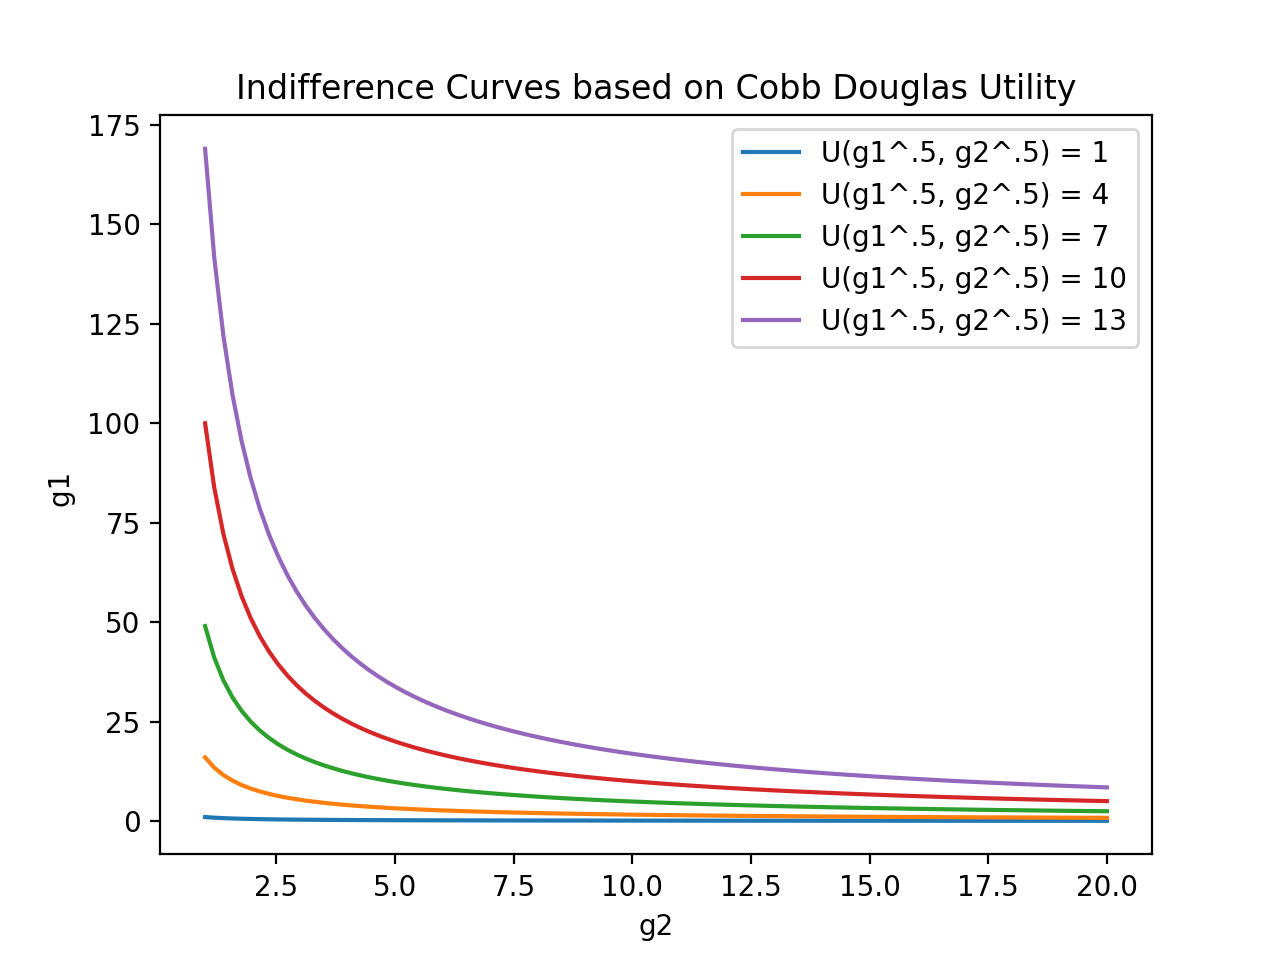
\includegraphics[width=3in, height=5.in]{Plots/indifference_curves.png}
\caption{A range of indifference curves without budget constraints.}
\end{marginfigure}

\subsection*{Optimising Utility}
A further complication arises when  we try to factor for a consumer's budget. The shape of the Cobb-Douglas function shows that the utility surface is constantly increasing with our rate acquisition. So without any constraints the consumer would not achieve satisfaction, but continue like glutton. But add a budget constraint and we need to find the maximum point at which an indifference curve insects with our budgetary line. Instead of solving the equation: 

$$ \text{ Find } g_{1}, g_{2} \text{ such that } u(g_{1}, g_{2}) = \lambda $$

\noindent we need to solve a constrained optimisation problem: 
$$ \text{ maximise } u(g_{1}, g_{2})  \text{ subject to } cost(g_{1}, g_{2}) =  \lambda$$

\noindent This style of problem can be approached with the method of Lagrange multipliers. If we let:

\begin{marginfigure}
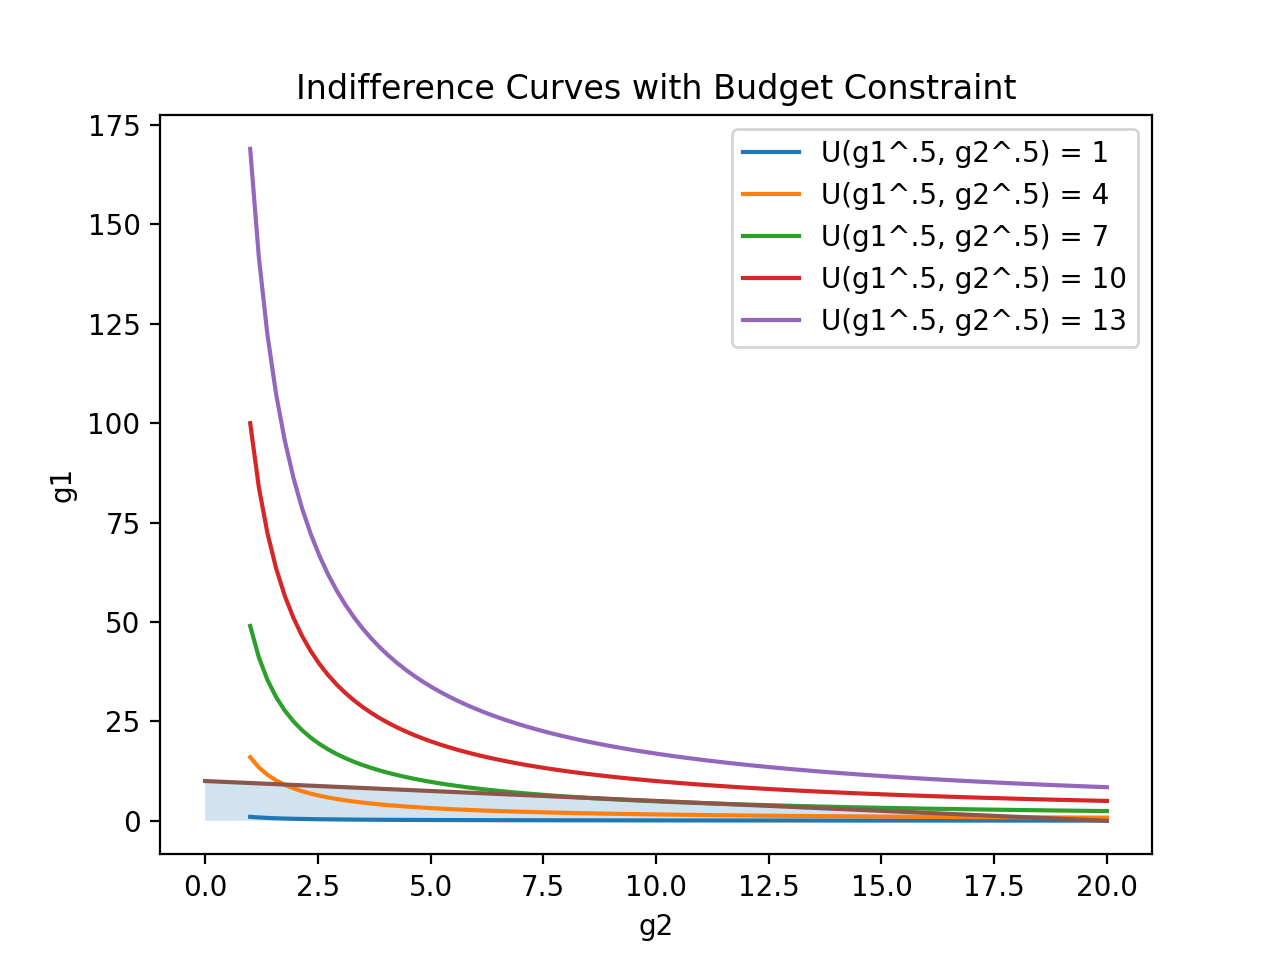
\includegraphics[width=3in, height=5.in]{Plots/indifference_curves_budget.png}
\caption{A range of indifference curves with budget constraints.}
\end{marginfigure}

$$ L = g_{1}^{\frac{1}{2}}g_{2}^{\frac{1}{2}} - \lambda(2g_{1} + 3g_{2} - 40) $$

\noindent where $2$ and $3$ are the unit cost of the respective goods, and $40$ is our total budget. While $\lambda$ is our Lagrangian multiplier. This term will be used to re-express the algebra of our equation as a function of the consumer's capacity to spend. We can discover where utility is maximised when the gradient of the curve can be set to zero. This is the theory behind the "hill climbing" algorithms of gradient descent. When the curvature of the "slope" has plateaued i.e. is zero, then we've reached a maximum or minimum in the multivariate space of the function. As before we want to use this fact to express the implicit function of $g_{1}$ in terms of $g_{2}$, but this time including the constraints.

\begin{fullwidth}
\begin{example}[  Lagrangian Multiplier]

\[
\nabla L = dL /  d\mathbf{g} =
    \begin{pmatrix}
       \dfrac{\partial u(\mathbf{g})}{\partial g_1}   & , \dfrac{\partial u(\mathbf{g})}{\partial g_2}
    \end{pmatrix} = \begin{pmatrix}
    \frac{1}{2}g_{1}^{-\frac{1}{2}}g_{2}^{\frac{1}{2} } - 2\lambda & ,
    \frac{1}{2}g_{2}^{-\frac{1}{2}}g_{1}^{\frac{1}{2} } - 3\lambda
    \end{pmatrix} = \mathbf{0}
  \]


$$ \Rightarrow \lambda = \frac{1}{4}g_{1}^{-\frac{1}{2}}\sqrt{g_{2}} = \frac{4}{25}g_{2}^{-\frac{1}{2}}\sqrt{g_{1}}$$

$$ \Rightarrow  (\frac{1}{4})^2\frac{1}{g_{1}}g_{2} = (\frac{4}{25})^2\frac{1}{g_{2}}g_{1} \Rightarrow (\frac{1}{4})^2 g_{2} = (\frac{4}{25})^2\frac{1}{g_{2}}g_{1}^2  \Rightarrow (\frac{1}{4})^2g_{2}^{2} = (\frac{4}{25})^2g_{1}^2 $$ 

$$ \Rightarrow g_{2} = \frac{16}{25}g_{1}$$

\noindent The same pattern holds for cases with more than two goods. We can express the value of given good $g_n$ in terms of a function $f(g_{1}, ... g_{n-1}) $. Then substituting this value into our constraint we get: 

$$ 2g_{1} + 3(\frac{16}{25})g_{1} = 40 \Rightarrow 2g_{1} + 1.92g_{1} = 40 \Rightarrow 3.92g_{1} = 40$$
Proving the optimial settings are  $g_{1}^{*} = 10.20 \text{ and } g_{2}^{*} = 6.52 \text{ and } \lambda^{*} = 0.20 $

\end{example}
\end{fullwidth}

This proof shows how we triangulate a consumer's view of any good as expressed through the medium of their utility function. But the method of Lagrangian multipliers is more than a mere algebraic trick. We can interpret the $\lambda$ term as the rate of change of the consumer's utility as a function of the cost. The proof is a little more involved, but the significance of this interpretation should be obvious. If we knew our consumer's adhered to a particular style of utility function we could model how price-changes would impact their returns to utility. 

\subsection*{From Indifference to Utility}

If we can elicit preference statements from our consumer we construct a utility curve as follows. First observe the preferences expressed by consumer decisions and then map the maximal and least preferred options to convenient polarities. For instance:

$$ g_{1} \succ g_{2} \succ g_{3} \succ g_{4} \succ g_{5} $$

\noindent where:

$$ u(g_{1}) = 0 \text{ and } u(g_{5}) = 1 $$

\noindent then each of the intermediary options can be measured in the interval between 0 and 1. However there are an infinite number of simple ordinal mappings that would work, and a strict ordering does nothing to convey the degree of feeling associated with each option. But we can calibrate utility scales based on decisions made about offered bets. Each individual good can be assessed against a simple win-loss lottery between the two most extreme outcomes. If the consumer is indifferent between the sure prospect of the good and a fixed odds lottery on their most preferred outcome, they've implicitly weighed their utility of the good. 

$$ \forall i \exists  p :  g _{i} \sim [p \cdot g_{1}, (1-p)\cdot g_{5}] \rightarrow u(g_{i}) = p $$

\noindent So whenever we are indifferent between a sure thing and a win-loss lottery over the best and worst outcomes we have implicitly chosen the utility of the of good on a 0-1 scale. In this manner we can construct a utility curve across the entire range of options. 

\section{Representation: Decision Under Risk}
The most famous result in decision theory is von Neumann and Morgenstern's Representation theorem. It shows using the technique discussed above how expressed preferences (which adhere to certain axioms of rationality) can track with a utility measure.  As such they can be interpreted as an agent's attempt to maximise their expected utility.  But the theorem is limited to decisions over well-defined lotteries, and as such makes a poor model for general choice under uncertainty where the odds are approximate. 

\begin{marginfigure}
\caption{Compound lotteries as probability trees}%
  
% Set the overall layout of the tree
\tikzstyle{level 1}=[level distance=3.5cm, sibling distance=3.5cm]
\tikzstyle{level 2}=[level distance=3.5cm, sibling distance=2cm]

% Define styles for bags and leafs
\tikzstyle{bag} = [text width=4em, text centered]
\tikzstyle{end} = [circle, minimum width=3pt,fill, inner sep=0pt]

% The sloped option gives rotated edge labels. Personally
% I find sloped labels a bit difficult to read. Remove the sloped options
% to get horizontal labels. 

\begin{tikzpicture}[grow=down, sloped]
\node[bag] {$[\frac{3}{7}Lot_{1}, \frac{4}{7}Lot_{2}]$}
    child {
        node[bag] {$[\frac{5}{9} g_{1}, \frac{4}{9} g_{2}]$}        
            child {
                node[end, label=
                    {[xshift=0.0cm, yshift=0.0cm]$\Big[ g_{1}(\frac{4}{7}\cdot\frac{5}{9})$}] {}
                edge from parent
                node[above] {$g_{1}$}
                node[below]  {$\frac{5}{9}$}
            }
            child {
                node[end, label=
                    {[xshift=0.0cm, yshift=0.0cm]$g_{2}(\frac{4}{7}\cdot\frac{4}{9}), $}] {}
                edge from parent
                node[above] {$g_{2}$}
                node[below]  {$\frac{4}{9}$}
            }
            edge from parent 
            node[above] {$Lot_{1}$}
            node[below]  {$\frac{4}{7}$}
    }
    child {
        node[bag] {$[\frac{6}{9}g_{3}, \frac{3}{9}g_{4}]$}        
        child {
                node[end, label=
                    {[xshift=0.0cm, yshift=0.0cm]$g_{3}(\frac{3}{7}\cdot\frac{6}{9}),$}] {}
                edge from parent
                node[above] {$g_{3}$}
                node[below]  {$\frac{6}{9}$}
            }
            child {
                node[end, label=
                    {[xshift=0.0cm, yshift=0.0cm]$g_{4}(\frac{3}{7}\cdot\frac{3}{9})  \Big] $}] {}
                edge from parent
                node[above] {$g_{4}$}
                node[below]  {$\frac{3}{9}$}
            }
        edge from parent         
            node[above] {$Lot_{2}$}
            node[below]  {$\frac{3}{7}$}
    };
\end{tikzpicture}

  \label{fig:compound lotteries}%
\end{marginfigure}

\begin{ftheo}{vNM's Representation Theorem}
If an individual i's preference relation $\succeq$ is transitive, complete and satisfies: \begin{enumerate}
\item (Continuity): $\forall g_{1} , g_{2} , g_{3} : ( g_{1} \succeq g_{2} \succeq g_{3}) \rightarrow \exists v \in [0, 1] \wedge g_{2} \sim_{i} [v g_{1}, (1-v) g_{3}]_{Lot}$
\item (Monotonicity): If $ v_{1}, v_{2} \in [0, 1]$ and $ g_{1} \succ g_{2}$ then  $ \Big( [ v_{1} g_{1}, (1-v_{1})g_{2}]_{Lot} \succeq [ v_{2} g_{1}, (1-v_{2})g_{2}]_{Lot} \Big) \Leftrightarrow v_{1} \geq v_{2}$
\item (Reduction of Compound lotteries): Each compound lottery ${[q_{1}Lot_{p_{1}}, ...,  q_{n}Lot_{p_{n}}]}$ reduces to a simple lottery where each good $(1, .. k)$ is weighted across all branches of the nested decision tree ${[(q_{1}p^{k}_{1} + q_{2}p^{k}_{2} ... + q_{n}p^{k}_{n})g_{k} .... , (q_{1}p^{k-1}_{1} , ...)g_{k-1} + ... (q_{1}p^{1}_{1} , ...)g_{1}]_{Lot}}$ by the usual rules of probability for branching compound events such that $\widehat{Lot} \sim Lot$ 
\item (Independence) If $\widehat{Lot} = [q_{1}Lot_{1}, ..., q_{j}Lot_{j}...q_{n}Lot_{n}]$ and $L_{j} \sim M$, then $\widehat{Lot} \sim \widehat{Lot}^{'} = [q_{1}Lot_{1}, ..., q_{j}M...q_{n}Lot_{n}]$ 
\end{enumerate}  
then $\exists u_{p} : [ g_{1}, ... g_{n}] \mapsto \text{ Val } $ where 
$ u_{p}(Lot) = p_{1}u(g_{1}) + ... + p_{k}u(g_{k}) = E(u_{p}(Lot))$ and  $u(g_{1}) \geq u(g_{2}) \Leftrightarrow g_{1} \succeq g_{2}$ so that $u$ represents $\succeq$ unique up to a positive linear transformation.
\end{ftheo}\footnote{We follow the example in: \cite{GameTheory}}

\noindent For a well defined and fixed probability function $p$ over the goods $g_{1} ..... g_{n}$ the above constraints are sufficient to define a sensible utility function based on an agent's expressed preferences. The thought gives hope to the idea that you would be able to predict an individual's actions in any environment where you knew both their preferences and the objective probabilities at play. This is the basic model for understanding poker play, the probabilities are generally known and it just remains to determine the game theoretical dynamics. 

\section{Representation: Decision Under Uncertainty}

\subsection*{From Neutrality to Desire}
One of the issues with eliciting a utility curve with appeals to bets over lotteries stems from the stigma associated with gambling. An alternative approach, more in the spirit of Bayesian philosophy is to try to elicit the desirability of a prospect by situating it between two polarities and repeatedly seeking a third prospect midpoint between the two, which is half as desirable by construction. The method, originally proposed by Frand Ramsey relies on the idea of an "Ethically Neutral" proposition $Neutral$ - one which if it exists is such that for all other prospects $\alpha$ we're utterly indifferent between: $$(Neutral \wedge \alpha) \sim \alpha \sim (\neg Neutral \wedge \alpha)$$. \noindent The idea is that we can gauge desire by offers of repeatededly refined contracts based on an ethically neutral proposition. This sequence of offers can be used to construct a utility curve. First observe that 

\begin{equation}
\begin{split}
[ \alpha \text{ if } Neutral, \omega \text{ if } \neg Neutral ]_{contract_{1}} \\  \sim [ \omega  \text{ if } Neutral, \alpha \text{ if } \neg Neutral ]_{contract_{2}} \\   \Rightarrow u(contract_{1})  = u(contract_{2})   \\  \Rightarrow EU(contract_{1}) \\ = u(\alpha)p(Neutral) + u(\omega)(1-p(Neutral)) \\ 
= u(\omega)p(Neutral) + u(\alpha)(1-p(Neutral)) \\ 
= EU(contract_{2})  
\\ \Leftrightarrow p(Neutral) = 0.5
\end{split}
\end{equation}

\noindent Then we can take any two extremes $u(\alpha) = 1, u(\omega) = 0$ and we can use our test for indifference to situate any third proposition $\gamma$ on a desirability scale since: 
\begin{equation} 
\begin{split}
 [\gamma \text{ if } Neutral, \gamma \text{ if } \neg Neutral]_{contract_1} \\ 
 \sim   [\alpha \text{ if } Neutral, \omega \text{ if } \neg Neutral ]_{contract_2} \\
 \Leftrightarrow EU(contract_{2}) = u(alpha)\frac{1}{2}  + u(omega)\frac{1}{2} = .5  \\ = u(\gamma) = EU(contract_{1})
\end{split}
\end{equation}

Repeating this step we can find a contract on a sure-thing $\psi$ for which we're indifferent between:
\begin{equation} 
\begin{split}
[\psi \text{ if } Neutral, \psi \text{ if } \neg Neutral]_{contract_1}  \\
 \sim   [\alpha \text{ if } Neutral, \gamma \text{ if } \neg Neutral ]_{contract_2} \\
  \Rightarrow u(\psi) = .75
   \\ . . . etc
 \end{split}
\end{equation}

Repeating this process indefinitely we can refine our utility scale as exactly as we please. If these measures adhere to certain basic constraints of rationality regarding consistency of utility we can show how a Bayesian agent can be seen to maximise their expected utility when making decisions under uncertainty. But unlike the Von Neumann representation theorem for a Bayesian perspective the probability function over prospects is not unique, we can have multiple pairs $\langle p, u \rangle$ which are representative of an individual's preference ordering $\succeq$ without converging on the particular probabilities ascribed by one individual. This is precisely the content of the following theorem. 

\begin{ftheo}{Bolker Representation Theorem}
\label{section:BolkersRepresentation}
Let $ \mathbb{B} =  \langle \Omega, \succeq \rangle $ be Bolker structure if $\Omega$ is an atomless Boolean algebra and $\models$ forms an implication relation over $\Omega$, while $\succeq$ is complete, transitive, continuous over $\Omega \setminus \bot$ and the following hold: 
\begin{enumerate}
\item (Impartiality) Suppose $\alpha \sim \beta $ and $\exists \gamma (\neg(\gamma \sim \alpha))$ such that  $\alpha \wedge \gamma = \bot = \beta \wedge \gamma$ and $\alpha \vee \gamma \sim \beta \vee \gamma $ Then $ \forall \gamma ( \alpha \vee \gamma \sim \beta \vee \gamma )$ 
\item (Averaging) If $\alpha \wedge \beta = \bot$ then $\alpha \succeq \beta \Leftrightarrow \alpha \succeq \alpha \vee \beta \succeq \beta$
\end{enumerate}
Then there is a probability measure and utility (desirability) metric $\langle p, u \rangle$ on $\Omega$ such that if the following axioms hold:
\begin{itemize}
\item (A0) $p(\top) = 1$
\item (A1) $p(\alpha) \geq 0$
\item (A2) $\alpha \wedge \beta = \bot \rightarrow p(\alpha \vee \beta) = p(\alpha) + p(\beta)$
\item (A3) $u(\top) = 0$
\item (A4) ${\alpha \wedge \beta = \bot \wedge p(\alpha \vee \beta) \neq 0}$  implies  ${u(\alpha \vee \beta) = \dfrac{u(\alpha)p(\alpha) + u(\beta)p(\beta)}{p(\alpha \vee \beta)} }$
\end{itemize}
it follows that
$$  u(\alpha) \geq u(\beta) \Leftrightarrow \alpha \succeq \beta $$

and there is another such set of functions $\langle p^{*}, u^{*}    \rangle$ if and only if $u^{*}$ is a fractional linear transformation of $u$ i.e. ${ \exists a > 0}$ and ${\exists c , cu(\alpha) > -1}$
$$ p^{*}(\alpha) = p(\alpha) \cdot (cu(\alpha) + 1) $$
$$u^{*}(\alpha) = \frac{au(\alpha)}{cu(\alpha)+1} $$
\end{ftheo}

The mathematical machinery used to prove this result is a little more involved, ranging over every possible boolean combination of beliefs measured on three axes: preference, probability and desirability. In addition to the usual probability axioms, (A3) and (A4) tie subjective probability and subjective utility together. The axiom (A3) works to normalise the utility scale so that no sure prospect has any positive utility. This, in a sense, enshrines the requirement that there is only a utility to novel information. While (A4) ensures that the utility of any disjunction is the weighted average of the ways in which it can occur. More importantly it implies:
 $$u(\alpha \vee \neg\alpha) = u(\top) = p(\alpha)u(\alpha) + p(\neg\alpha)u(\neg\alpha)$$  
 $$= p(\alpha)u(\alpha) + u(\neg\alpha) - p(\alpha)u(\neg\alpha) $$
 $$ \Rightarrow u(\top) - u(\neg\alpha) = p(\alpha)u(\alpha)  - p(\alpha)u(\neg\alpha)$$
 $$ \Rightarrow p(\alpha) = \frac{u(\top) - u(\neg\alpha)}{ u(\alpha)  - u(\neg\alpha)} \text{  if } u(\alpha) \neq u(\neg\alpha) $$ 
Which confirms how the relationship between probability of a given proposition can be expressed in terms of the desirability or utility of the same proposition and it's negation. 
So $\alpha \sim \beta \succeq \top \succeq \neg\alpha \sim \neg\beta$
\newline

\noindent The criteria of (Impartiality) and (Averaging) are less transparent. Averaging has some intuitive appeal if we consider two inconsistent propositions, say $\alpha$ = ``Arsenal win the Premier League'' and  $\beta$ =``Manchester United win the Premier League''.  If we're Arsenal fans is stands to reason that our preference $\alpha \succeq \beta$ should imply that we prefer the win  ($\alpha$) to the possibility ($\alpha \vee \beta)$ of the win over the loss ($\beta$).  
 
\noindent For impartiality the argument is a little different. Suppose $\alpha, \beta $ is as above but we're Chelsea supporters. Let $\gamma$ = ``Chelsea wins the Premier League'' then if you are indifferent between the possibilities $\alpha \vee \gamma \sim \beta \vee \gamma$ it must be because you consider $\alpha , \beta$ equally probable. Hence it follows that you should be indifferent between choices over disjunctions of $\alpha, \beta$ and any third choice $\gamma$. The importance of this axiom in the uniqueness proof stems from the fact that given one pair of propositions about which we're indifferent this supplies an explicit test for ranking propositions by probability and more generally the ratio of probabilities. From this ranking combined with the above axioms (A0 - A4) Jeffrey can infer the probability scale and a desirability measure from our preferences. 

\bibliography{sample-handout}
\bibliographystyle{plainnat}



\end{document}
